\chapter{Литературный обзор} \label{ch:ch1}

%------------------------------------------------------------------------------------------
\section{Удаление меркаптанов} \label{sec:ch1/sec1}

Меркаптаны, или, согласно более точному термину, тиолы, представляют собой класс органических соединений, содержащих группу $SH$. Их структурная формула обычно записывается как $RSH$, где $R$ может представлять собой алкильную или ароматическую группу. Меркаптановые компоненты обычно содержаться в природном газе и жидком топливе, таких как бензин, керосин, дизельное топливо. Необходимость удаления меркаптанов обусловлена несколькими факторами:
	1234
\begin{enumerate}
	\item Их кислые свойства могут привести к серьезным проблемам с коррозией;
	\item Неприятный запах, обусловленный наличием меркаптанов, требует их удаления из топлива перед сжиганием;
	\item Большинство меркаптанов обладают высокой токсичностью.
\end{enumerate}

Меркаптаны преимущественно представлены низкомолекулярными $C _1$ – $C _3$ прямо-цепными соединениями в составе ПГ и СУГа, в то время как в более тяжелых фракциях присутствуют разветвленные и более высокомолекулярные меркаптаны. Исследования по обработке топлива, содержащего меркаптаны, начались в 1860 году, и традиционные методы удаления основаны на использовании неорганических солей, первый метод «метод докторской очистки» описан в патенте \cite{kalinowski_doctor_1959}. и второй метод так называемая «медная очистка» \cite{krause_color_1952}. В этих методах меркаптаны не удаляются из топлива, а превращаются в дисульфиды, которые не проявляют коррозионную активность и обладают относительно незначительным запахом. Следовательно, содержание серы в топливе не снижается в результате самой очистки обоими упомянутыми традиционными методами.

Метод докторской очистки, который является наиболее старым из них, основан на использовании соли свинца: плумбита натрия ($Na_2PbO_2$). На первом этапе раствор $Na_2PbO_2$, полученный путем растворения оксида свинца в растворе гидроксида натрия ($NaOH$), смешивается с топливом, подлежащим обработке. Меркаптаны в топливе реагируют с $Na_2PbO_2$, образуя свинцовый меркаптид ($(RS)_2Pb$), который растворяется в топливе по реакции \cref{eq:reaction1}:

\begin{equation}
	\mathrm{Na_2PbO_2 + 2RSH \rightarrow {(RS)_2Pb} + 2NaOH} \label{eq:reaction1}
\end{equation}

$(RS)_2Pb$ может быть вновь превращен в $Na_2PbO_2$ с использованием воздуха по реакции \cref{eq:reaction2}: 

\begin{equation}
	\mathrm{(RS)_2Pb + 2NaOH + 1/2O_2 \rightarrow RSSR + Na_2PbO_2 + H_2O} \label{eq:reaction2} 
\end{equation} 

Однако восстановление раствора $Na_2PbO_2$ этим методом происходит медленно и лишь частично. Для полного превращения $(RS)_2Pb$ в дисульфид $(RSSR)$ в реакционную смесь добавляется молекулярная сера, и $(RS)_2Pb$ полностью превращается в свинцовый сульфид $(PbS)$, который выпадает из раствора по реакции \cref{eq:reaction3}:

\begin{equation}
	\mathrm{(RS)_2Pb + S \rightarrow RSSR + PbS} \label{eq:reaction3}
\end{equation} 

Этот процесс обеспечивает полное превращение, однако свинцовый сульфид не может быть восстановлен, поэтому его необходимо утилизировать при завершении реакции. Более того, поскольку сера, добавленная в реакционную смесь для образования дисульфидов, сама растворяется в топливе, содержание серы увеличивается после обработки. В связи с этим данный процесс редко применяется сегодня, за исключением случаев аналитического использования, включенный в стандарты ASTM (ASTM D 4952-09) \cite{noauthor_doctor_nodate}.

Еще один традиционный метод превращения меркаптанов, который называется «медной очисткой» в котором медь используется в виде хлорида ($CuCl_2$). На первом этапе меркаптаны окисляются до дисульфидов по реакции \cref{eq:reaction4}:

\begin{equation}	
	\mathrm{2RSH + 2CuCl_2 \rightarrow RSSR + 2CuCl + 2HCl} \label{eq:reaction4}
\end{equation}

Затем суспензию хлорида меди $(I)$ окисляют снова до хлорида меди $(II)$ с помощью воздуха, в соответствии с реакцией \cref{eq:reaction5}:
\begin{equation}	
	\mathrm{2CuCl + 2HCl + 1/2O_2 \rightarrow 2CuCl_2 + 2H_2O} \label{eq:reaction5}
\end{equation}

Хотя эти процессы все еще используются в некоторых областях, технологии, которые описываются далее, обычно предпочтительнее с точки зрения производительности и затрат.

Существует два основных способа обработки больших объемов меркаптанов в углеводородном сырье: экстракция, где легкие меркаптаны окисляются и удаляются в виде дисульфидов, и очищение, где тяжелые меркаптаны также окисляются, но остаются в потоке. Эти методы применяются при удалении \num{200} кг серы эквивалентов и более в день. Для потоков с меньшим количеством меркаптанов (менее \num{200} кг серы эквивалентов в день) используются альтернативные методы, такие как промывка.

Два основных поставщика лицензий на процессы удаления больших количеств меркаптанов - UOP (Merox\cite{farshi_kinetic_2005}) и GTP-Merichem (Merichem\cite{kohl_gas_1997}). В зависимости от характеристик необходимой степени очистки сырья, каждая компания использует различные конфигурации процессов \cite{bricker_advances_2012, noauthor_mericat_nodate, noauthor_thiolex_nodate}, что отображено в Таблице \cref{tab:remove}.

\begin{table}
	\centering
	\fontsize{12}{15}\selectfont % Установка размера шрифта
	\captionsetup{justification=centering} % выравнивание подписи по-центру
	\caption{Процессы удаления меркаптанов с большим их содержанием \cite{de_angelis_natural_2012}.}\label{tab:remove}
	\begin{tabular}{lllllc}
		\toprule
		Сырье   & Макс. содержание & Процесс      & Процесс    & Содержание после &  \\
		        & до обработки     & Merox        & Merichem   & обработки        &  \\
		        & (ppm Серы)       &              &            &                  &  \\ \midrule
		ПГ      & \num{10000}      & Merox        & Merichem   & Сокращение       &  \\
		СУГ     &                  & Абсорбция,   & Абсорбция, &                  &  \\
		        &                  & Экстракция   & Экстракция &                  &  \\
		Нафта   & \num{5000}       & Экстракция   & Экстракция & Неизменная       &  \\
		бензин  &                  & fixed bed    &            &                  &  \\
		        &                  & sweetening,  &            &                  &  \\
		        &                  & Minalk       &            &                  &  \\
		        &                  & sweetening   &            &                  &  \\
		Нафта   & \num{1000}       & fixed bed    & fixed bed  & Неизменная       &  \\
		Керосин &                  & sweetening,  & sweetening &                  &  \\
		ДТ      &                  & caustic free &            &                  &  \\
		        &                  & sweetening   &            &                  &  \\ \bottomrule
	\end{tabular}
\end{table}

Перед каждым применением процессов Merox или Merichem необходима предварительная щелочная очистка с разведенным раствором гидроксида натрия ($NaOH$), чтобы удалить весь $H_2S$ в сырье. При этом содержание $H_2S$ не должно превышать \num{10} ppm, так как в противном случае $H_2S$ может необратимо реагировать с сильными щелочными растворами, используемыми в процессах Merox или Merichem. Процессы Merox имеют более широкое распространение и масштабы, превышающие \num{1,8} млн. тонн в сутки. К январю \num{2002} года введено в эксплуатацию почти \num{1600} установок с производительностью от \num{5,5} до \num{19,096} тонн в сутки. Для обработки тяжелого сырья, такого как нефть, керосин, дизельное топливо и отопительные масла, также необходима предварительная щелочная очистка для удаления нафтеновых кислот.

Для обработки легкого углеводородного сырья, таких как ПГ или  СУГ, содержащие в себе низкомолекулярные меркаптаны (от метилмеркаптана до бутилмеркаптана), применяются процессы абсорбции и экстракции. На первом этапе газовый поток взаимодействует с концентрированным раствором гидроксида натрия (10-20\% массовой концентрации $NaOH$), в котором меркаптаны растворяются в виде соответствующих натриевых солей по реакции \cref{eq:reaction6}:

\begin{equation}
	\label{eq:reaction6}
	\mathrm{RSH_\text{(газофазная или жидкофазная)} + NaOH \rightarrow RSNa_\text{(жидкофазная)}} 
\end{equation}

На первом этапе процесса, который осуществляется в колонном аппарате, меркаптаны взаимодействуют с щелочным раствором противотоком, в результате чего ПГ или СУГ проходит через верхнюю часть колонны. Вода, содержащая меркаптаны в виде натриевых солей, а также катализатор Merox или Merichem (комплекс фталоцианина кобальта), вытекает из нижней части колонны, затем подогревается и направляется на окисление в регенератор. В регенераторе щелочной раствор реагирует с воздухом, что приводит к окислению меркаптидов до дисульфидов по реакции \cref{eq:reaction7}:

\begin{equation}	
	\mathrm{4RSNa + O_2 + 2H_2O \rightarrow 2RSSR + 4NaOH} \label{eq:reaction7}
\end{equation}

Дисульфиды формируют новую маслянистую фазу, которая тяжелее воды, и эта двухфазная смесь направляется в сепаратор. После этого регенерированный щелочной раствор возвращается в колонну разделения, а маслянистая фаза направляется на соответствующие нужды, например, использование дисульфидного масла как сульфидирущего агента для катализатора гидроочистки, ингибитор коксообразования УЗК и при возможности, продажа как химического реагента. При использовании данных процессов периодически добавляется небольшое количество катализатора для поддержания достаточной эффективности процесса. При обработке методом абсорбции или экстракции меркаптаны превращаются в менее агрессивные и токсичные дисульфиды, а так же и содержание серы в газе уменьшается, поскольку образовавшиеся при окислении меркаптанов дисульфиды удаляются. Прямые операционные расходы оцениваются в \num{4,6} рублей за \num{1} кубический метр очищенного ПГ и \num{230} рублей за \num{1} кубический метр для очистки СУГ.

В таблицах \cref{tab:solid, tab:liquid} приведены наиболее распространенные хемосорбционные процессы для очистки углеводородного сырья в которых содержится малое количество сернистых соединений \cite{foral_evaluation_1995} (обычно менее \num{200} ppm, в пересчете на общую серу) с использованием твердых и жидких поглотителей. Большинство процессов представляют собой стехиометрические реакции между молекулами, содержащими серу, и реагентом, который не может быть восстановлен и должен быть утилизирован. Обычная аминовая очистка (МЕА, ДЕА и МДЕА) не являются экономически выгодными. Эти процессы предназначены для использования, где ежедневное производство соединений серы не превышает \num{185} кг серы в день.  

\begin{table}
	\centering
	\fontsize{12}{15}\selectfont % Установка размера шрифта
	\captionsetup{justification=centering} % выравнивание подписи по-центру
	\caption{Процессы для небольшого количества $H_2S$ и меркаптанов (твердая фаза)\cite{abdulrahman_natural_2012, kohl_gas_1997, de_angelis_natural_2012}.} \label{tab:solid}
	\begin{tabular}{lllllc}
		\toprule
		Название процесса & Активная        & Вид           & Возможность & Максимальная &  \\
		(компания)        & фаза            & процесса      & рецикла     & произв.,     &  \\
		                  &                 &               &             & кг/день      &  \\ \midrule
		Iron sponge       & Оксид железа на & Периодический & нет         & \num{45}     &  \\
		(Connelly-GPM)    & опилках дерева  &               &             &              &  \\
		Sulfatreat        & Гематит         & Периодический & нет         & \num{90}     &  \\
		(Sulfatreat)      &                 &               &             &              &  \\
		Sulphur-Rite      & Оксид железа    & Fixed bed     & нет         & \num{180}    &  \\
		(Merichem)        &                 &               &             &              &  \\
		Low temperature   & Оксид цинка     & Fixed bed     & нет         & \num{135}    &  \\
		zinc oxide (ICI)  &                 &               &             &              &  \\
		Chemsweet         & Оксид цинка +   & Периодический & нет         & \num{18}     &  \\
		(NATCO)           & ацетат цинка    &               &             &              &  \\
		Sulfosorb         & Активный уголь  & Fixed bed     & да          & \num{1,4}    &  \\
		(Calgon           & насыщенный      &               &             &              &  \\
		carbon co.)       & солями меди     &               &             &              &  \\ \bottomrule
	\end{tabular}
\end{table}

\begin{table}
	\centering
	\fontsize{12}{15}\selectfont % Установка размера шрифта
	\captionsetup{justification=centering} % выравнивание подписи по-центру
	\caption{Процессы для небольшого количества $H_2S$ и меркаптанов (жидкая фаза) \cite{de_angelis_natural_2012}.} \label{tab:liquid}
	\begin{tabular}{lllllc}
		\toprule
		Название процесса & Активная            & Вид           & Возможность & Максимальная &  \\
		(компания)        & фаза                & процесса      & рецикла     & произв.,     &  \\
		                  &                     &               &             & кг/день      &  \\ \midrule
		Sulfa-check       & Водный раствор      & Периодический & нет         & \num{90}     &  \\
		(Nalco-Exxon)     & $NaNO_2$            &               &             &              &  \\
		Sulfascrub        & 50\% водный раствор & Периодический & нет         & \num{45}     &  \\
		(Petrolite Co.)   & триазина            &               &             &              &  \\
		The Eliminator    & Раствор триазина    & Периодический & нет         & \num{90}     &  \\
		(Merichem)        &                     &               &             &              &  \\ \bottomrule
	\end{tabular}
\end{table}

%------------------------------------------------------------------------------------------
\subsection{Аппаратурное оформление процесса демеркаптанизации.} \label{sec:ch1/sec2}

Процесс удаления меркаптанов из СУГ может быть реализован различными способами, и выбор конкретного метода зависит от требований качества очистки, объемов обрабатываемого газа, экономической целесообразности и других факторов. На рисунке \cref{fig:ExtPlus} изображена схема экстракции процесса Merox "Extractor Plus" \cite{bricker_advances_2012}.

\begin{figure}
	\centering
	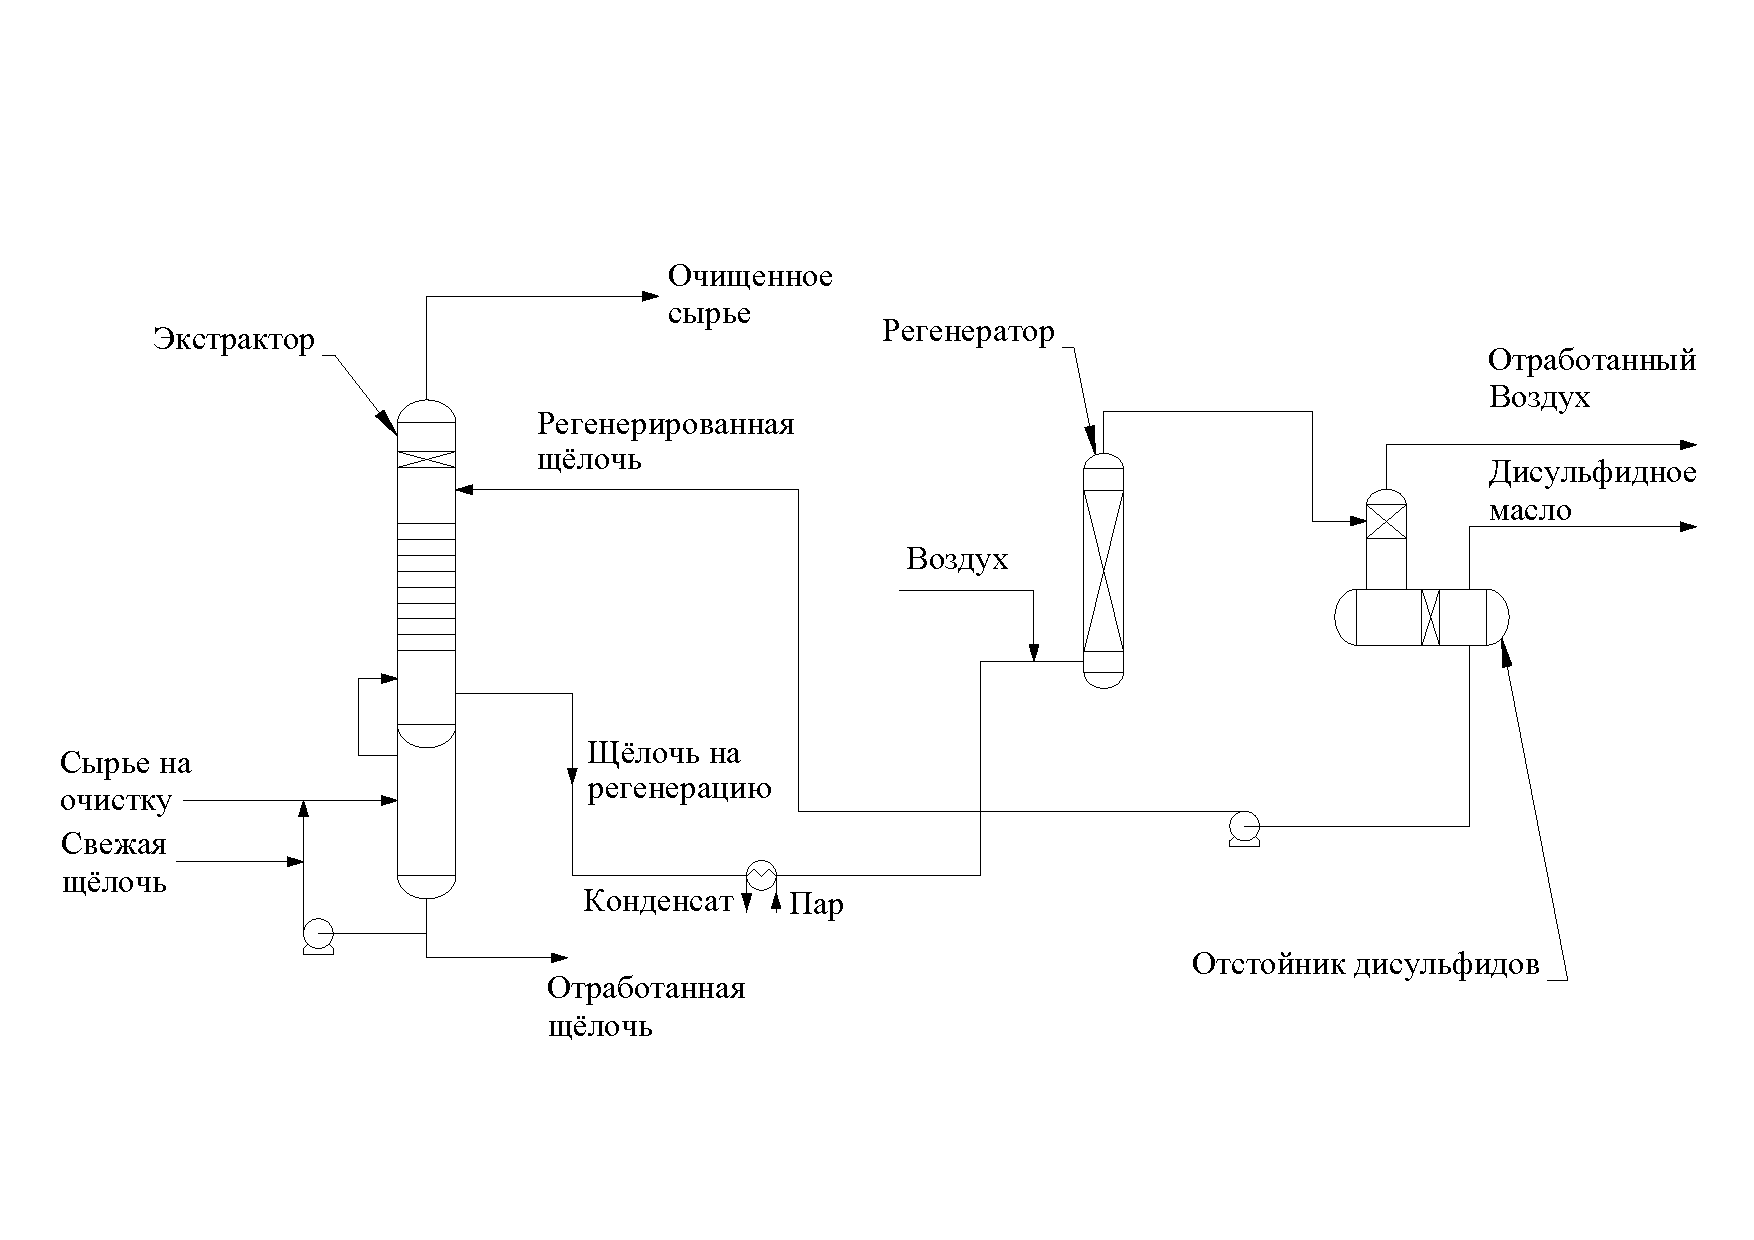
\includegraphics[width=1\linewidth]{images/Extplus}
	\caption{Схема демеркаптанизации компании Merox (Extractor Plus).}
	\label{fig:ExtPlus}
\end{figure}

Это стандартное предложение UOP, где удаление проводят в противоточном тарельчатом либо насадочном экстракторе, данная схема обеспечивает эффективное удаление меркаптановой серы из СУГ. На первом этапе в кубе колонны проводят предварительную очистку сырья с наибольшим содержанием меркаптанов с использованием свежей щелочи для удаления остаточного $H_2S$. Затем, поднимаясь вверх по колонне, сырье которое уже содержит в себе меньше меркаптанов контактирует с регенерированным щелочным раствором. Для обеспечения необходимого уровня удаления меркаптанов рассчитывают необходимый слой насадки или количество тарелок. Противоток в экстракторе обеспечивает благоприятное условие равновесия реакции \cref{eq:reaction6}. В верхней части колонны предусмотрен каплеотбойник для предотвращения уноса щелочи, а из куба колонны насыщенная меркаптидами щелочной раствор поступает на регенерацию. 

Регенерация щелочи осуществляется в отдельной колонне по реакции \cref{eq:reaction7}. Данную окислительную реакцию проводят с избытком воздуха в присутствии катализатора (Merox WSTM), реакция протекает только в сторону образования продукта и более высокая температура до \num{70}°C способствует увеличению скорости реакции. Merox WSTM - это гомогенный катализатор фталоцианина кобальта, который позволяет восстановить щелочной раствор путем окисления меркаптидов до дисульфидов. Отработанный воздух сепарируется из отстойника дисульфидов, а дисульфидное масло отправляется на нужды потребителю, регенерированная щелочь с малым содержанием меркаптидов возвращается в экстрактор.

\begin{figure}
	\centering
	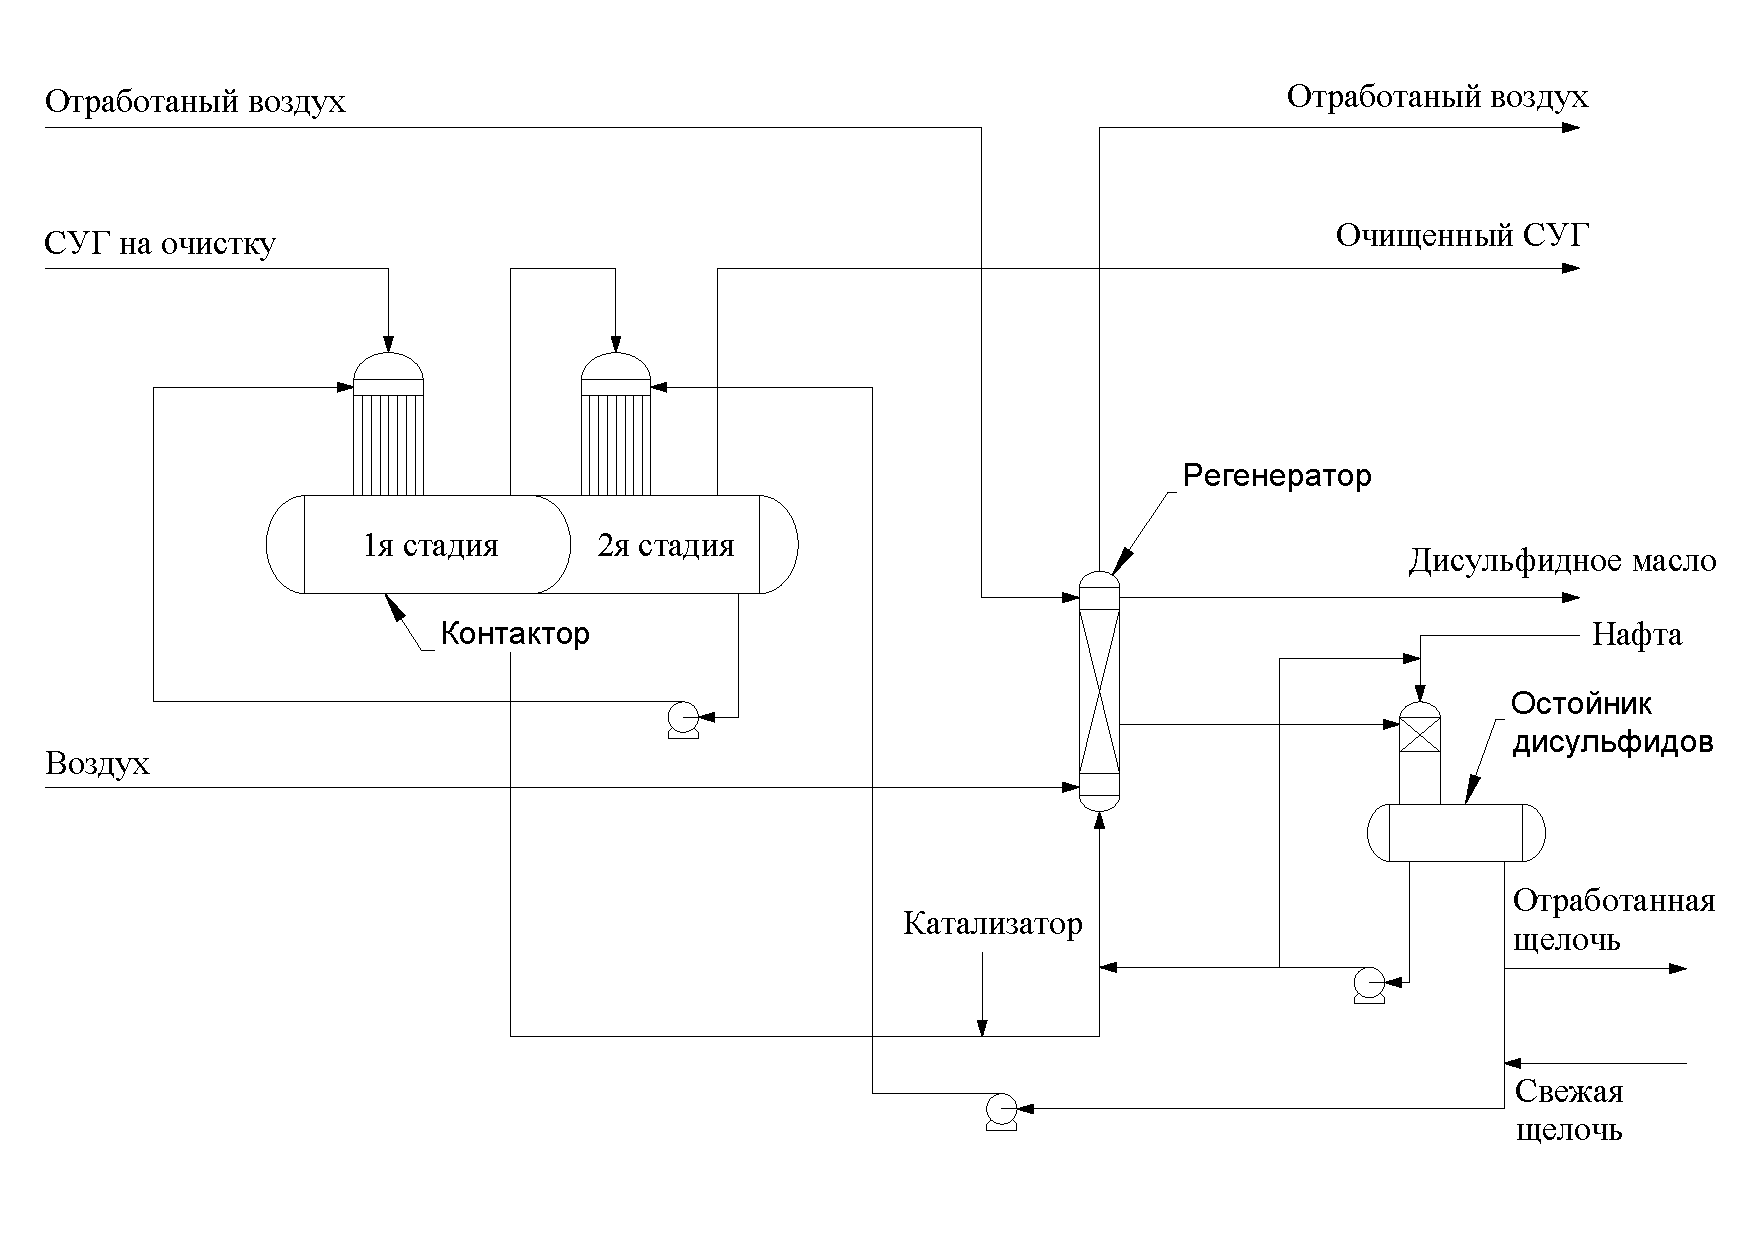
\includegraphics[width=1\linewidth]{images/Eth}
	\caption{Схема двухсекционной демеркаптанизации компании Merichem (THIOLEX).}
	\label{fig:THIOLEX}
\end{figure}

\begin{figure}
	\centering
	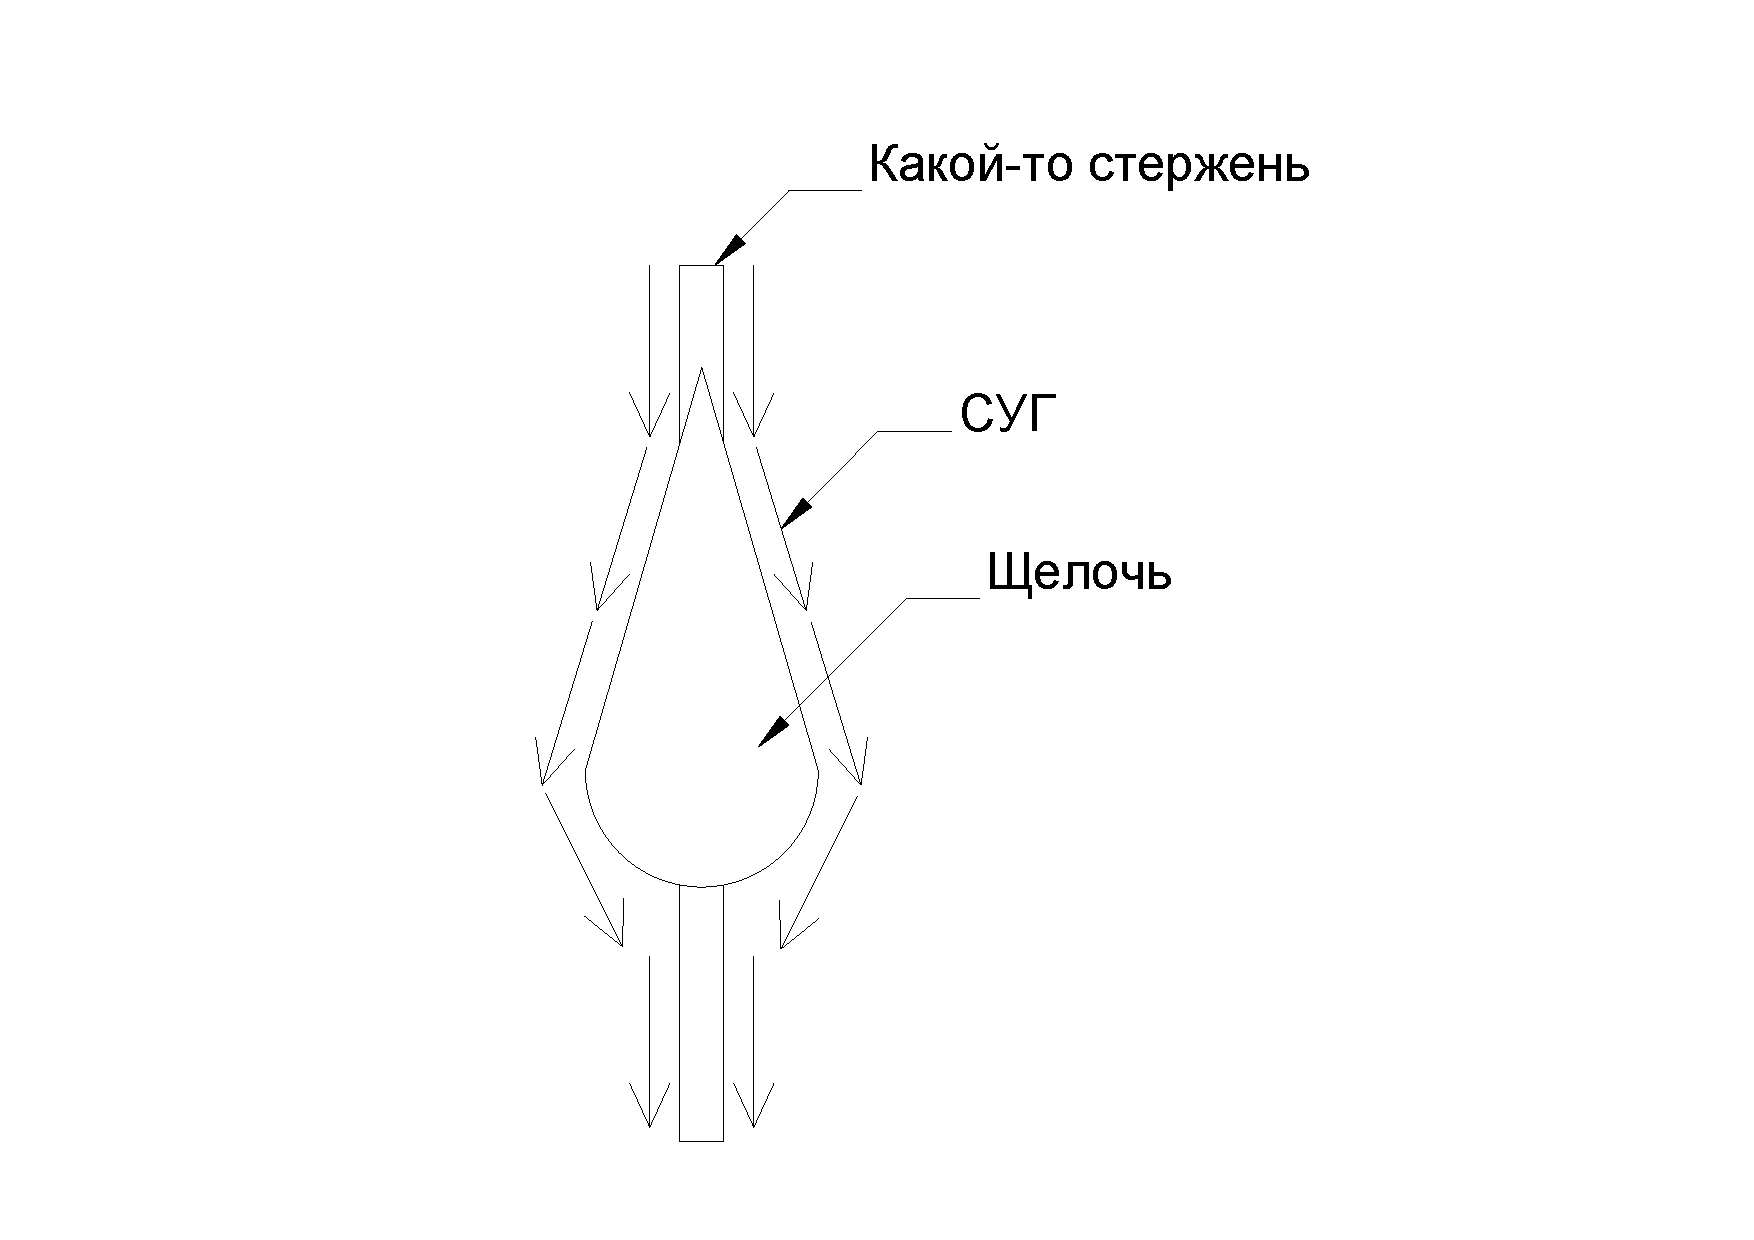
\includegraphics[width=0.6\linewidth]{images/fibr}
	\caption{Схема работы фиброволокнистого контактного устройства компании Merichem.}
	\label{fig:FIBERFILM}
\end{figure}

Так же стоит отметить предложение от компании Merichem рисунок \cref{fig:THIOLEX}, 
процесс THIOLEX, демеркаптанизацию проводят в двухсекционном отстойнике, где щелочная раствор смачивает фиброволокнистое контактное устройство рисунок \cref{fig:FIBERFILM}, затем СУГ стекает по смоченному щелочью контактному устройству и на поверхности раздела фаз реагирует с ней, $H_2S$ и меркаптаны переходят щелочную фазу в виде сульфидов и меркаптидов натрия. Обе фазы отделяются друг от друга в двухсекционном отстойнике, насыщенный сульфидами и меркаптидами натрия щелочной раствор выводится с нижней части отстойника и под собственным давлением направляется на регенерацию, а очищенный до \num{10} ppm c первой секции СУГ поступает на доочистку во вторую секцию отстойника и очищается до \num{5} ppm, так же отмечено что происходит унос щелочного раствора до \num{0,1} ppm. Регенерацию проводят в колонне, где насыщенный щелочной раствор с гомогенным катализатором поднимаясь верх по колонне контактирует с воздухом и происходит окисление содержащихся в щелочном растворе сульфидами и меркаптидами натрия до дисульфидов. Для снижения плотности дисульфидного масла, с целью облегчения его отделения от щелочного раствора в отстойнике дисульфидов, в отстойник подается расчетное количество нафты. Дисульфидное масло с более низким значением плотности, выводится из колонны регенератора для отгрузки на потребительские нужды.

%-----------------------------------------------------------------------------------------------------
\subsection{Влияние контактных устройств на гидродинамику и массообмен процесса.} \label{sec:ch1/sec3}

Схема противоточной системы хемосорбцонной экстракции из двух (частично) растворимых друг в друге жидкостей СУГ и водно-щелочной раствор представлена на рисунке \cref{fig:cheme}.

\begin{figure}
	\centering
	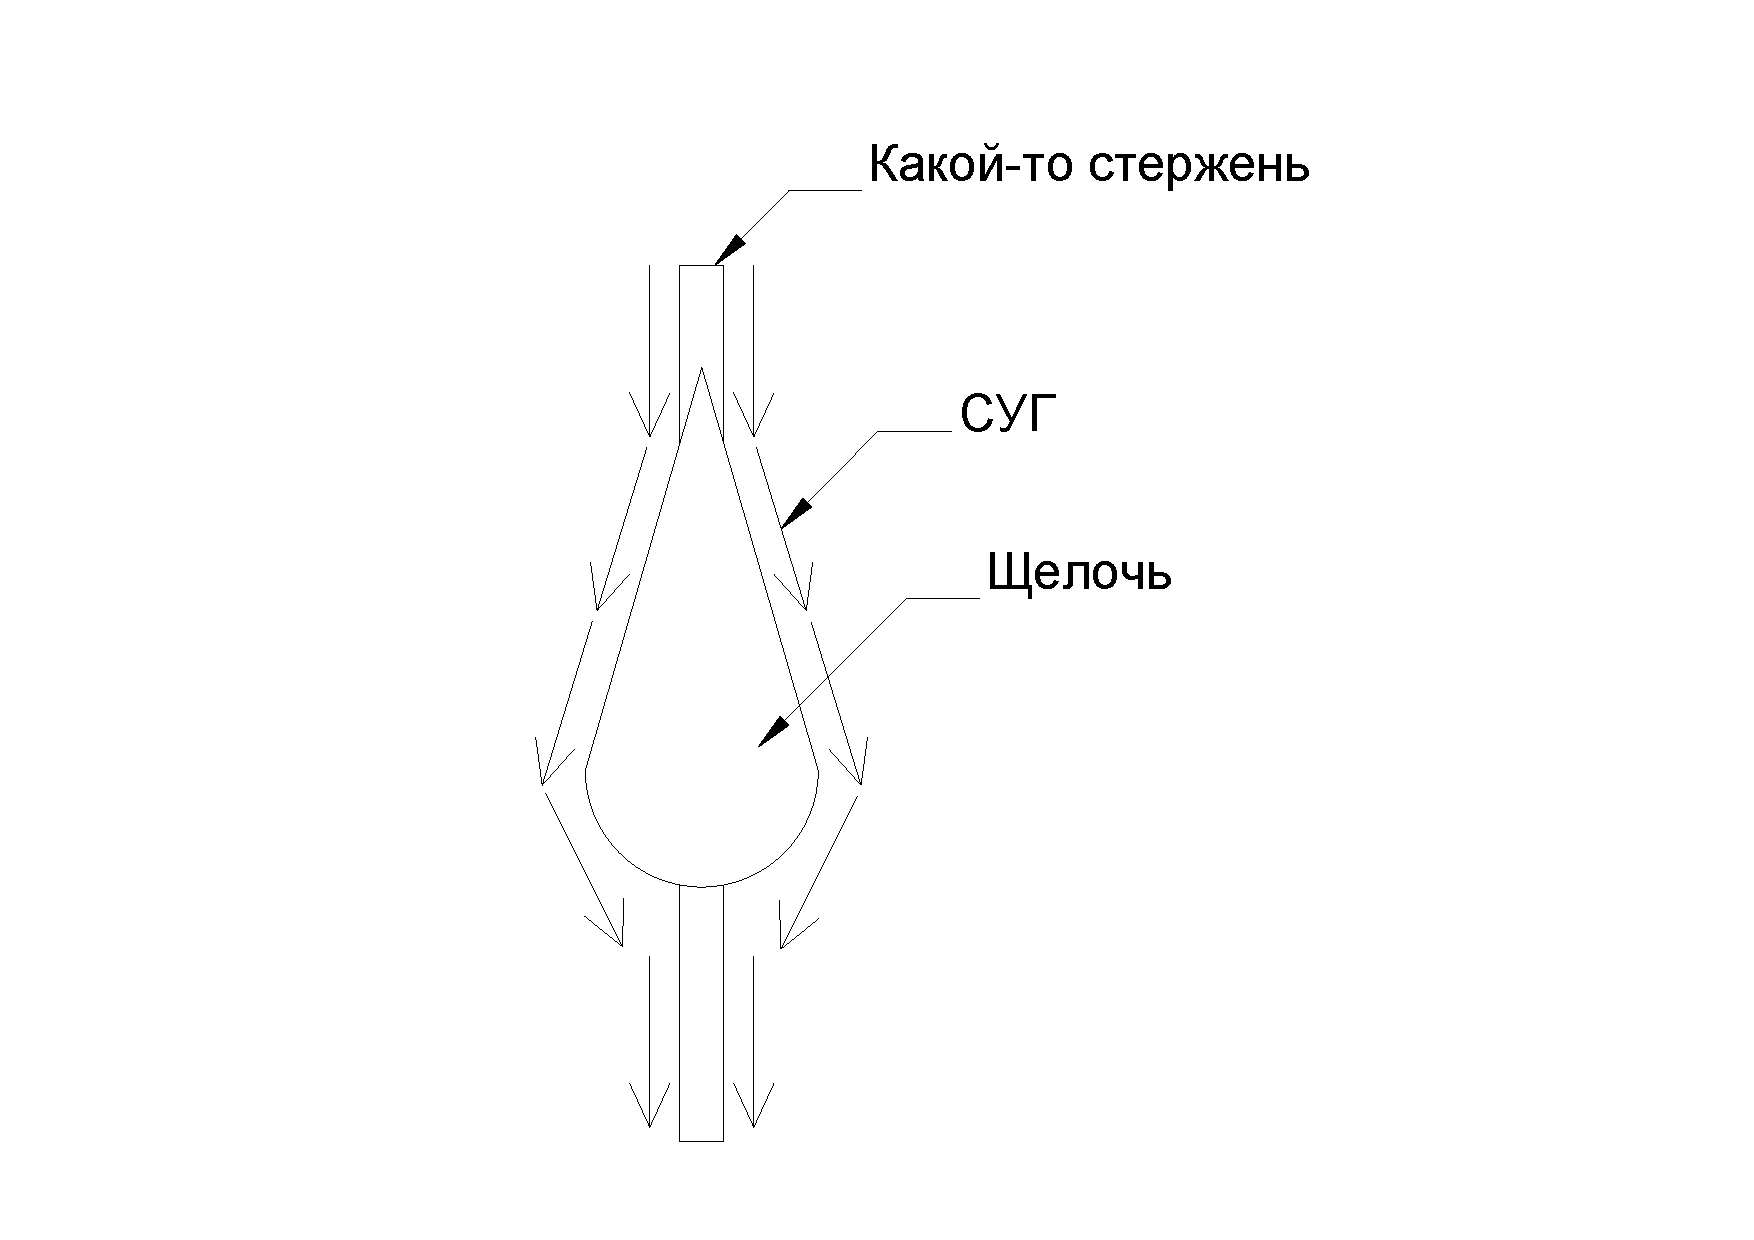
\includegraphics[width=0.6\linewidth]{images/fibr}
	\caption{Заглушка.}
	\label{fig:cheme}
\end{figure}

Взаимодействие фаз в процессе демеркаптанизации может происходить как ступенчато, так и непрерывно. Процесс ступенчатого взаимодействия осуществляется в смесительно-отстойных аппаратах \cref{fig:THIOLEX}, в то время как непрерывное взаимодействие происходит в колонных аппаратах \cref{fig:ExtPlus}. В колоннах противоточное движение фаз осуществляется за счет действия силы тяжести, вызванной разницей плотностей фаз.

Колонные аппараты характеризуются низкой эффективностью из-за ограниченной поверхности контакта фаз, обусловленной большими размерами капель. Кроме того, в аппаратах с размерами более $1,5$ метров наблюдаются значительные поперечные неравномерности (масштабные эффекты), что приводит к снижению эффективности разделения смеси.

Одним из распространенных аппаратов для процесса демеркаптанизации являются колонны с ситчатыми тарелками. В них водно-щелочная фаза заполняет всю колонну и перемещается с тарелки на тарелку, тогда как другая дисперсная фаза (СУГ) диспергируется через отверстия на тарелках, перемещается в пространстве между тарелками и, достигая следующей тарелки, коалесцирует. Этот процесс диспергирования и коалесцирования происходит многократно, увеличивая интенсивность процесса демеркаптанизации. Присутствие ситчатых тарелок способствует уменьшению обратного перемешивания. Также применяются аппараты с насадкой, пульсационные и вибрационные аппараты.

 
\subsection{Диффузионные процессы химической технологии.} \label{sec:ch1/sec4}

Диффузионные процессы, при которых меняется состав обеих фаз, выгодно проводить по принципу

В химической технологии большое значение имеют процессы диффузионного обмена веществом между фазами. Сюда относятся процессы абсорбции (поглощения газов жидкостями) и экстракции (перенос вещества между двумя несмешивающимися жидкими фазами). Поглощение газа жидкостью подобно процессу конденсации, с той лишь разницей, что к диффузионному сопротивлению газа добавляется диффузионное сопротивление конденсированной фазы. Если абсорбция не сопровождается медленными химическими реакциями, то на поверхности устанавливается равновесие между концентрациями диффундирующего вещества в газовой и жидкой фазах. При стационарном протекании процесса он может быть описан моделью двух пленок: газовой и жидкой. Как и всегда в подобных случаях, действует закон сложения последовательным сопротивлений \cref{eq:equation1}:
 
\begin{equation}
	\label{eq:equation1}
	\begin{alignedat}{2}
		j_1 = \frac{xC^0_\text{газ} - C^0_\text{жидкость}}{\frac{1}{\beta_\text{жидкость}} + \frac{x}{\beta_\text{газ}}} = \frac{C^0_\text{газ} - \frac{C^0_\text{жидкость}}{x}}{{\frac{1}{\beta_\text{жидкость}} + \frac{1}{x\beta_\text{ж}}}}
	\end{alignedat}
\end{equation}\\
где x - равновесная растворимость;

Величины, стоящие в знаменателе, представляют собой диффузионные сопротивления газовой и жидкой пленок, отнесенные к концентрациям либо в жидкой, либо в газовой фазе.

Диффузионные процессы, при которых меняется состав обеих фаз, выгодно проводить по принципу противотока: газ и жидкость поступают с противоположных концов аппарата (газ снизу, жидкость сверху). Таким образом используется наибольшая доступная разность концентраций. При расчете противоточных процессов удобно ввести понятие теоретической тарелки пли ступени переноса. При этом непрерывный процесс переноса приближенно заменяется ступенчатым и принимается, что на каждой ступени устанавливается равновесие между фазами. Необходимое число теоретических тарелок находится простым графическим методом: строится диаграмма, в которой по двум осям отложены концентрации рассматриваемого компонента в двух фазах. На этой диаграмме проводятся линия равновесия по закону растворимости и рабочая линия по уравнению материального баланса. Ступенчатый процесс представляется на диаграмме ломаной, прямоугольные ступеньки которой лежат между линией равновесия и рабочей линией. Число теоретических тарелок равно числу ступенек этой линии. 

В тарельчатых колоннах необходимое число действительных тарелок находится умножением числа теоретических тарелок на коэффициент полезного действия тарелки, находимый раз навсегда экспериментальным. В насадочных колоннах (скрубберах) опреде-ляется экспериментально длина насадки, эквивалентная одной теоретической тарелке. В аппаратах с пробулькивапием (барбoтажем) из эксперимента находится высота подъема пузырьков, эквивалентная теоретической тарелке. 

Метод теоретических тарелок позволяет, таким образом, для противоточных аппаратов обойти расчет самого диффузионного процесса: он заменяется расчетом равновесия, дополненным эмпирическими коэффициентами. Если известны коэффициенты переноса, то длину, эквивалентную одной теоретической тарелке, или коэффициент полезного действия можно рассчитать. Для тарельчатых колонн естественным представляется нестационарный метод расчета коэффициента полезного действия, подробно разработанный Кишиневским [8]. В этом методе рассматривается нестационарпый процесс диффузии для жидкой частицы за время ее пребывания на тарелке, без пользования понятием приведенной пленки. Для насадочиых колонн успешно применяется стационарный метод расчета в приближении двойной пленки; при этом число теоретических тарелок выражается через число единиц переноса (ЧЕП), которое, согласно формуле (III, 38а), связано с критерием Стэптопа. Изложение этого вопроса можно найти в монографии Рамма [9], к которой и отсыпаем интересующегося читателя. Анализ, учитывающий процессы не только диффузии, но и теплолередачи, дал Жаворопков [10]. 

